
\begin{figure}
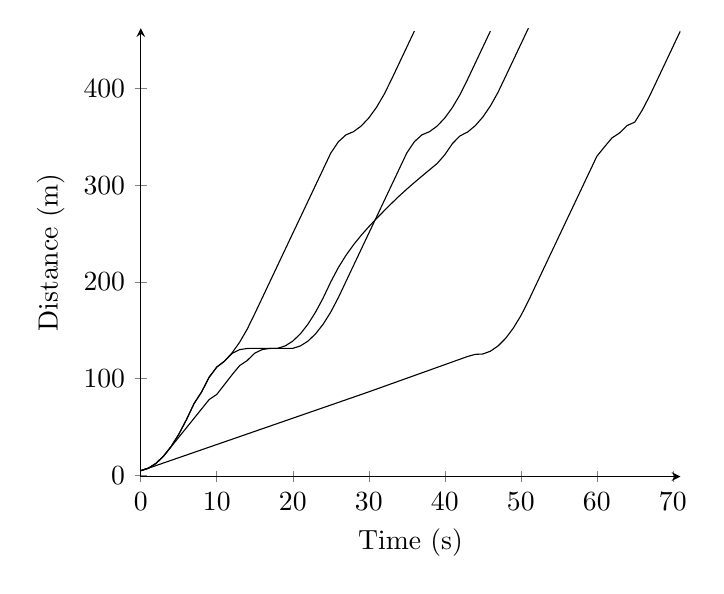
\begin{tikzpicture}
\begin{axis}[
legend style={anchor=west},
axis x line=bottom,
axis y line=left,
ymin=-1,
xlabel=Time (s),
ylabel=Distance (m),
]
\addplot[] coordinates {
(0, 5.1)
(1, 7.6)
(2, 12.6)
(3, 20.1)
(4, 30.1)
(5, 42.6)
(6, 57.6)
(7, 74.2)
(8, 86.34)
(9, 101.632252112)
(10, 112.059454389)
(11, 118.089689106)
(12, 126.619923822)
(13, 137.650158538)
(14, 151.180393254)
(15, 167.210627971)
(16, 183.810627971)
(17, 200.410627971)
(18, 217.010627971)
(19, 233.610627971)
(20, 250.210627971)
(21, 266.710627971)
(22, 283.310627971)
(23, 299.910627971)
(24, 316.510627971)
(25, 333.110627971)
(26, 344.787518658)
(27, 351.915724023)
(28, 355.232982832)
(29, 361.050241642)
(30, 369.367500452)
(31, 380.184759262)
(32, 393.502018071)
(33, 409.319276881)
(34, 425.919276881)
(35, 442.519276881)
(36, 459.119276881)
};
\addplot[] coordinates {
(0, 5.1)
(1, 7.6)
(2, 12.6)
(3, 20.1)
(4, 29.8362617914)
(5, 39.573371168)
(6, 49.3115981405)
(7, 59.0513413305)
(8, 68.7932151601)
(9, 78.5382194357)
(10, 83.8280997709)
(11, 93.9040106676)
(12, 103.981624555)
(13, 113.52705814)
(14, 118.801600362)
(15, 126.48300364)
(16, 130.230000938)
(17, 131.303895816)
(18, 131.399242419)
(19, 131.399242419)
(20, 131.399242419)
(21, 133.899242419)
(22, 138.899242419)
(23, 146.399242419)
(24, 156.399242419)
(25, 168.899242419)
(26, 183.899242419)
(27, 200.499242419)
(28, 217.099242419)
(29, 233.699242419)
(30, 250.299242419)
(31, 266.799242419)
(32, 283.399242419)
(33, 299.999242419)
(34, 316.599242419)
(35, 333.195903477)
(36, 344.843825685)
(37, 351.946271708)
(38, 355.24383803)
(39, 361.041404351)
(40, 369.338970673)
(41, 380.136536994)
(42, 393.434103316)
(43, 409.231669637)
(44, 425.831669637)
(45, 442.431669637)
(46, 459.031669637)
};
\addplot[] coordinates {
(0, 5.1)
(1, 7.6)
(2, 12.6)
(3, 20.1)
(4, 30.1)
(5, 42.6)
(6, 57.6)
(7, 74.2)
(8, 86.34)
(9, 101.632252112)
(10, 112.059454389)
(11, 118.089689106)
(12, 126.079818867)
(13, 130.071924431)
(14, 131.27865093)
(15, 131.398797075)
(16, 131.398797075)
(17, 131.398797075)
(18, 131.398797075)
(19, 133.898797075)
(20, 138.898797075)
(21, 146.398797075)
(22, 156.398797075)
(23, 168.898797075)
(24, 183.473930824)
(25, 200.073930824)
(26, 214.896631075)
(27, 227.519643186)
(28, 238.444329628)
(29, 248.143178411)
(30, 257.015075616)
(31, 265.367166701)
(32, 273.300911563)
(33, 281.147558725)
(34, 288.741937109)
(35, 295.857053676)
(36, 302.674840662)
(37, 309.319997452)
(38, 315.868920083)
(39, 322.365638461)
(40, 331.362356839)
(41, 342.859075217)
(42, 350.840888311)
(43, 354.826344749)
(44, 361.311801186)
(45, 370.297257624)
(46, 381.782714061)
(47, 395.768170499)
(48, 412.253626936)
(49, 428.853626936)
(50, 445.453626936)
(51, 462.053626936)
};
\addplot[] coordinates {
(0, 5.1)
(1, 7.6)
(2, 10.3181088707)
(3, 13.0362604242)
(4, 15.7544574928)
(5, 18.4727031654)
(6, 21.1910008172)
(7, 23.909354144)
(8, 26.6277672007)
(9, 29.3462444467)
(10, 32.0647907972)
(11, 34.7834116835)
(12, 37.5021131223)
(13, 40.2209017973)
(14, 42.9397851542)
(15, 45.6587715127)
(16, 48.3778701993)
(17, 51.0970917043)
(18, 53.8164478702)
(19, 56.5359521168)
(20, 59.2556197146)
(21, 61.9754681158)
(22, 64.6955173598)
(23, 67.4157905739)
(24, 70.1363145934)
(25, 72.8571207407)
(26, 75.5782458086)
(27, 78.2997333169)
(28, 81.0216351331)
(29, 83.7440135908)
(30, 86.49254491)
(31, 89.2946863182)
(32, 92.1021686967)
(33, 94.9097494427)
(34, 97.7174486395)
(35, 100.52529232)
(36, 103.333314885)
(37, 106.141562837)
(38, 108.950100757)
(39, 111.759021335)
(40, 114.568463211)
(41, 117.37864516)
(42, 120.189938662)
(43, 123.003046572)
(44, 125.18372143)
(45, 125.567712567)
(46, 128.451703704)
(47, 133.835694841)
(48, 141.719685978)
(49, 152.103677115)
(50, 164.987668253)
(51, 180.37165939)
(52, 196.97165939)
(53, 213.57165939)
(54, 230.17165939)
(55, 246.77165939)
(56, 263.37165939)
(57, 279.87165939)
(58, 296.47165939)
(59, 313.07165939)
(60, 329.67165939)
(61, 339.382345387)
(62, 348.78013274)
(63, 353.929949201)
(64, 361.579765663)
(65, 365.079582124)
(66, 377.729398586)
(67, 392.879215047)
(68, 409.479215047)
(69, 426.079215047)
(70, 442.679215047)
(71, 459.279215047)
};

\end{axis}
\end{tikzpicture}
\label{tik:distance:100:81}
\caption{100 percent diving with GSC on route $81$}
\end{figure}
